\begin{pastexam}[label={px:gw3-108-ds-01}]{關務三等資訊處理 108 年 第一題}
（申論；20 分）

下列程式函式 doit()以 C 語言語法呈現，用以對雙向鏈結串列（doubly linked list）進行處理。請依據該函式回答問題。
\begin{minted}[fontsize=\small]{c}
void doit(struct node **head){
     struct node *temp = NULL;
     struct node *current = *head;

     while(current != NULL){
          temp = current->prev;
          current->prev = current->next;
          current->next = temp;
          current = current->prev;
     }

     if(temp != NULL)
          *head = temp->prev;
}
\end{minted}
\begin{enumerate}[leftmargin=2.2em]
\item[㈠] 若 X 指向一個雙向鏈結串列如下，其中 X->prev 指向 NULL，X->next 指向資料為 21 的節點。請顯示並
說明 doit（\&X）執行過後該串列變化結果。（10 分）
\begin{center}
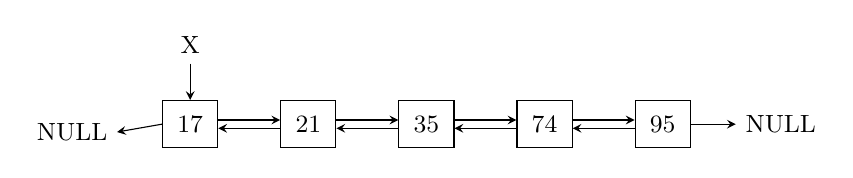
\begin{tikzpicture}[>=stealth, nd/.style={draw, minimum width=7mm, minimum height=6mm, font=\small}]
\foreach \v [count=\k] in {17,21,35,74,95}{ \node[nd] (n\k) at (1.5*\k,0) {\v}; }
\foreach \a/\b in {1/2,2/3,3/4,4/5}{
  \draw[->] ([yshift=1.5pt]n\a.east) -- ([yshift=1.5pt]n\b.west);
  \draw[->] ([yshift=-1.5pt]n\b.west) -- ([yshift=-1.5pt]n\a.east);
}
\node[font=\small] (L) at (0,-0.1) {NULL};
\node[font=\small] (R) at (9,0) {NULL};
\draw[->] (n1.west) -- (L.east);
\draw[->] (n5.east) -- (R.west);
\node[font=\small] (X) at (1.5,1) {X};
\draw[->] (X) -- (n1.north);
\end{tikzpicture}
\end{center}
\item[㈡] 若 X 指向一個雙向鏈結串列如下，其中 X->prev 指向資料為 17 的節點，X->next 指向資料為 35 的節點。
請顯示並說明 doit（\&X）執行過後該串列的變化結果。（5 分）
\begin{center}
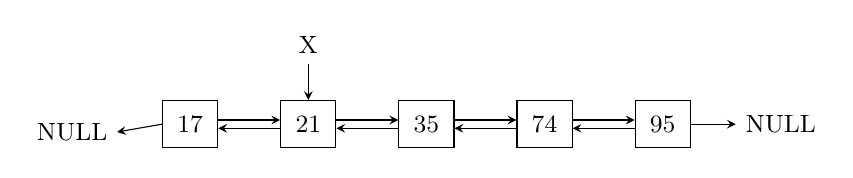
\begin{tikzpicture}[>=stealth, nd/.style={draw, minimum width=7mm, minimum height=6mm, font=\small}]
\foreach \v [count=\k] in {17,21,35,74,95}{ \node[nd] (n\k) at (1.5*\k,0) {\v}; }
\foreach \a/\b in {1/2,2/3,3/4,4/5}{
  \draw[->] ([yshift=1.5pt]n\a.east) -- ([yshift=1.5pt]n\b.west);
  \draw[->] ([yshift=-1.5pt]n\b.west) -- ([yshift=-1.5pt]n\a.east);
}
\node[font=\small] (L) at (0,-0.1) {NULL};
\node[font=\small] (R) at (9,0) {NULL};
\draw[->] (n1.west) -- (L.east);
\draw[->] (n5.east) -- (R.west);
\node[font=\small] (X) at (3,1) {X};
\draw[->] (X) -- (n2.north);
\end{tikzpicture}
\end{center}
\item[㈢] 若 X 指向一個環狀雙向鏈結串列（circular doubly linked list），請說明 doit（\&X）是否仍能順利執行。
（5 分）
\end{enumerate}
\end{pastexam}

\begin{pastsoln}
\textbf{函式在做什麼。} 迴圈對 \texttt{current} 所指的節點交換 \texttt{prev} 和 \texttt{next}（\texttt{temp}
暫存舊的 \texttt{prev}），然後 \texttt{current = current->prev}：交換之後的 \texttt{prev} 就是\textbf{原本的}
\texttt{next}，所以 \texttt{current} 沿原本的方向往後走，直到走出串列（\texttt{NULL}）。 迴圈結束時
\texttt{temp} 是最後一個節點原本的 \texttt{prev}，也就是倒數第二個節點；它交換後的 \texttt{prev} 是原本的
\texttt{next}，就是最後一個節點，所以 \texttt{*head = temp->prev} 讓 head 指向原本的最後一個節點。 整體效果：
從 head 開始往後的每個節點都把兩個指標對調，head 改指原本的尾端，也就是\textbf{反轉雙向鏈結串列}
（資結書第~5.2、5.5~節）。 \texttt{temp} 為 \texttt{NULL} 表示串列是空的或只有一個節點，head 不用改。

\textbf{㈠ 串列被反轉，X 指向 95。} 逐輪追蹤（每列是一輪做完的狀態；「prev/next」是該節點交換後的值）：
\begin{center}
\begin{tabular}{ccccc}
\toprule
輪 & 處理的節點 & \texttt{temp} & 交換後 prev / next & 下一個 \texttt{current} \\
\midrule
1 & 17 & NULL & 21 / NULL & 21 \\
2 & 21 & 17 & 35 / 17 & 35 \\
3 & 35 & 21 & 74 / 21 & 74 \\
4 & 74 & 35 & 95 / 35 & 95 \\
5 & 95 & 74 & NULL / 74 & NULL \\
\bottomrule
\end{tabular}
\end{center}
迴圈結束時 \texttt{temp} 指向 74，74 的 \texttt{prev} 現在是 95，所以 \texttt{X = 95}。 結果：
\begin{center}
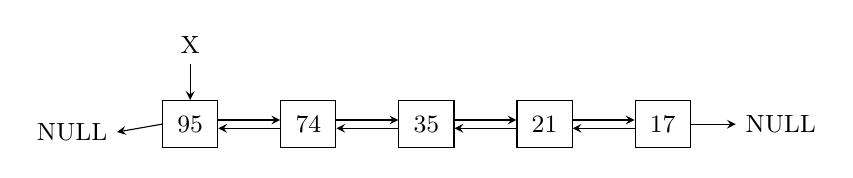
\begin{tikzpicture}[>=stealth, nd/.style={draw, minimum width=7mm, minimum height=6mm, font=\small}]
\foreach \v [count=\k] in {95,74,35,21,17}{ \node[nd] (n\k) at (1.5*\k,0) {\v}; }
\foreach \a/\b in {1/2,2/3,3/4,4/5}{
  \draw[->] ([yshift=1.5pt]n\a.east) -- ([yshift=1.5pt]n\b.west);
  \draw[->] ([yshift=-1.5pt]n\b.west) -- ([yshift=-1.5pt]n\a.east);
}
\node[font=\small] (L) at (0,-0.1) {NULL};
\node[font=\small] (R) at (9,0) {NULL};
\draw[->] (n1.west) -- (L.east);
\draw[->] (n5.east) -- (R.west);
\node[font=\small] (X) at (1.5,1) {X};
\draw[->] (X) -- (n1.north);
\end{tikzpicture}
\end{center}
從 X 沿 \texttt{next} 走是 95, 74, 35, 21, 17；95 的 \texttt{prev} 和 17 的 \texttt{next} 是 NULL。 仍是一個正確的
雙向鏈結串列，只是順序反過來。

\textbf{㈡ 只有 21 以後的部分被反轉，17 沒動，串列被弄壞。} 這次從 21 開始，17 在 X 前面，迴圈碰不到它：
\begin{center}
\begin{tabular}{ccccc}
\toprule
輪 & 處理的節點 & \texttt{temp} & 交換後 prev / next & 下一個 \texttt{current} \\
\midrule
1 & 21 & 17 & 35 / 17 & 35 \\
2 & 35 & 21 & 74 / 21 & 74 \\
3 & 74 & 35 & 95 / 35 & 95 \\
4 & 95 & 74 & NULL / 74 & NULL \\
\bottomrule
\end{tabular}
\end{center}
結束時同樣 \texttt{X = temp->prev = 95}。 各節點的指標變成：
\begin{center}
\begin{tabular}{ccc}
\toprule
節點 & prev & next \\
\midrule
95 & NULL & 74 \\
74 & 95 & 35 \\
35 & 74 & 21 \\
21 & 35 & 17 \\
17 & NULL & 21（沒改） \\
\bottomrule
\end{tabular}
\end{center}
\begin{center}
\begin{tikzpicture}[>=stealth, nd/.style={draw, minimum width=7mm, minimum height=6mm, font=\small}]
\foreach \v [count=\k] in {95,74,35,21,17}{ \node[nd] (n\k) at (1.5*\k,0) {\v}; }
\foreach \a/\b in {1/2,2/3,3/4,4/5}{
  \draw[->] ([yshift=1.5pt]n\a.east) -- ([yshift=1.5pt]n\b.west);
}
\foreach \a/\b in {1/2,2/3,3/4}{
  \draw[->] ([yshift=-1.5pt]n\b.west) -- ([yshift=-1.5pt]n\a.east);
}
\draw[->] (n5.south) to[out=-120, in=-60] node[below, font=\scriptsize] {17 的 next 仍指向 21} (n4.south);
\node[font=\small] (L) at (0,-0.1) {NULL};
\draw[->] (n1.west) -- (L.east);
\node[font=\small] (R) at (9,0.9) {NULL};
\draw[->] (n5.north) -- (R);
\node[font=\scriptsize] at (9.3,0.5) {17 的 prev};
\node[font=\small] (X) at (1.5,1) {X};
\draw[->] (X) -- (n1.north);
\end{tikzpicture}
\end{center}
從 X 沿 \texttt{next} 走：95, 74, 35, 21, 17, 21, 17, \dots，21 和 17 的 \texttt{next} 互指，永遠走不到 NULL；
而 17 的 \texttt{prev} 是 NULL，21 的 \texttt{prev} 卻是 35，兩個方向不一致。 這已經不是合法的雙向鏈結串列。
原因是 doit 假設傳進來的是串列的\textbf{第一個}節點（\texttt{prev} 為 NULL）。

\textbf{㈢ 不能，會變成無窮迴圈。} 環狀串列裡沒有任何指標是 NULL，\texttt{current} 永遠不會變成 NULL。
具體來說，第一圈把每個節點的指標都對調，處理完最後一個節點後，它原本的 \texttt{next} 是 X，\texttt{current}
回到 X；第二圈再對調一次等於還原，而且方向反過來沿原本的 \texttt{prev} 走；之後一圈反轉、一圈還原，
迴圈不會結束，函式不會回傳。 要反轉環狀雙向串列，迴圈條件要改成「回到起點就停」，例如先處理 X，再
\texttt{while (current != X)} 處理其他節點，最後讓 head 指向原本 X 的 \texttt{prev}。
\end{pastsoln}
